Per quanto riguarda la presenza di contenuto sgradito all'utente:
	\begin{itemize}
		\item \textbf{Pop-up}: presente. Nello specifico viene aperto un pop-up che informa l'utente dell'utilizzo di cookie: \\ 
								\begin{center}
\begin{figure}[h!]
           \begin{center}
           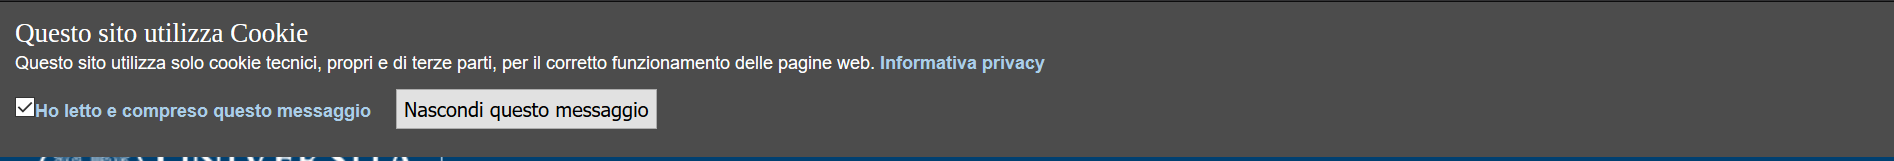
\includegraphics[scale=0.40]{C:/Users/elepo/Desktop/UNI/WIM/ANALISI_SITO/Relazione/sez/cookie.png}
           \caption{Cookie}
           \end{center}
  \end{figure}
\end{center}
		\item \textbf{Richieste d'uso di plugin}: non presente;
		\item \textbf{Apertura indesiderata di contenuti audio/video}: non presente;
		\item \textbf{Pubblicità}: non presente;
		\item \textbf{Registrazione forzata}: non presente.
	\end{itemize}